Per la misurazione della saturazione di ossigeno del sange è necessario implementare una formula per il calcolo. Essa si basa sulle differenze di tensione rilevate con luce rossa e con luce IR. Si valuta il rapporto $R$ tra l’assorbimento della componente rossa e infrarossa, secondo la formula seguente
\begin{equation}
    R=\frac{\left(\frac{AC}{DC}\right)_{RED}}{\left(\frac{AC}{DC}\right)_{IR}}=\frac{\frac{\left(V_{\text{max},RED}-V_{\text{min},RED}\right)}{V_{\text{min},RED}}}{\frac{\left(V_{\text{max},IR}-V_{\text{min},IR}\right)}{V_{\text{min},IR}}}
\end{equation}
A partire da R, è possibile calcolare il livello di saturazione utilizzando la formula riportata in Figura \ref{fig:GraphO2}
\begin{figure}[H]
    \centering
    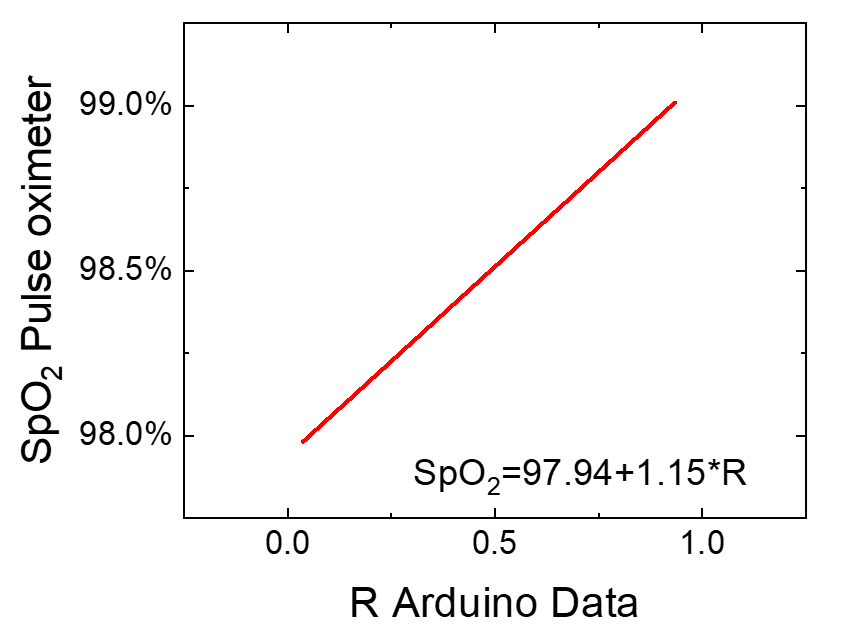
\includegraphics[width=0.7\linewidth]{GraphO2.png}
    \caption{$SpO_2$ pulse oximeter}
    \label{fig:GraphO2}
\end{figure}
\begin{lstlisting}[frame=single, language=Arduino]
float findO2(int array[]){
    int samples = 1000;
    int IR[samples];
    int RED[samples];
    digitalWrite(PinIR,HIGH);
    delay(250);
    for(int i = 0; i < samples; i++){
        IR[i] = analogRead(sensorPin);
        delay(1);
    }
    digitalWrite(PinIR,LOW);
    delay(100);
    digitalWrite(PinRED,HIGH);
    delay(250);
    for(int i = 0; i < samples; i++){
        RED[i] = analogRead(sensorPin);
        delay(1);
    }
    digitalWrite(PinRED,LOW);

    float k = 0.00080586;

    float IRmax = findmax(IR) * k;
    float IRmin = findmin(IR) * k;
    float REDmax = findmax(RED) * k;
    float REDmin = findmin(RED) * k; 

    float R = ((REDmax - REDmin)/REDmin) / ((IRmax - IRmin) / IRmin);
    float O2 = 97.94 + 1.15 * R;
    
    tft.setCursor(30, 280);
    tft.print("O2: ");
    tft.print(O2);
    
    return O2;
}
\end{lstlisting}